\chapter{Results} \label{ch:results}

This chapter presents the results of conducting experiments under the methodology proposed in Chapter \ref{ch:methodology}. The experiments were designed to evaluate the performance of the implemented \acrshort{drl} models for portfolio optimisation in changing environment representations and market conditions. Moreover, to analyse the interpretability of the model's decisions, a framework using post-hoc explainability techniques is explored.

\section{Dataset} \label{sec:dataset}

Given the general difficulty in finding the appropriate \acrshort{drl} algorithm with a suitable \gls{rewardfunction} for portfolio optimisation, the five implemented algorithms were tested on five different datasets. Each dataset consists of a different set of financial assets, ranging from three different asset classes. First, three datasets were constructed using the stock constituents of three renowned indexes:
\begin{itemize}
    \item \acrfull{djia} with 30 stocks,
    \item \acrfull{eurostoxx50} with 50 stocks,
    \item \acrfull{ftse100} with 100 stocks.
\end{itemize}

The constituents of each of the indexes were retrieved in April 2025 and can be found in Appendix \ref{sec:datasets-equities}. It is important to note that the datasets were chosen to illustrate different currencies, as this introduces another factor of changing market conditions. 

Additionally, two datasets were constructed using commodities and currencies, respectively. The commodities dataset includes six different commodities, which are listed in Appendix \ref{sec:datasets-commodities}. These are a sample of the most traded commodities in the market and were chosen by their availability in the \texttt{Yahoo! Finance API} \footnote{https://uk.finance.yahoo.com}. With regard to the currencies dataset, it includes ten different currency pairs, listed in Appendix \ref{sec:datasets-currencies}. These were selected based on their trading volume and liquidity, with all pairs quoted in \acrfull{usd}.

The datasets are constructed using daily data from January 2016 to July 2025 downloaded using the Python \texttt{yfinance} library \cite{yfinance}. The dataset is partitioned into two disjoint sets: training and testing, with the training set containing data from January 2016 to December 2023, and the testing set starting on January 2024 until July 2025. The training set is used to train the \acrshort{drl} models, while the testing set is used to evaluate their performance. For hyper-parameter tuning, the training set is further split into a training and validation set, with the validation set corresponding to the period between January 2023 and December 2023. The validation set is used to evaluate the performance of the models for each hyper-parameter combination. The train-validation-test split is summarised in Table \ref{tab:dataset-split}.

\begin{longtable}{|l|l|l|l|}
    \hline
    \textbf{Dataset} & \textbf{Training Period} & \textbf{Validation Period} & \textbf{Testing Period} \\
    \hline
    DJIA & Jan 2016 - Dec 2022 & Jan 2023 - Dec 2023 & Jan 2024 - Jul 2025 \\
    \hline
    Euro Stoxx 50 & Jan 2016 - Dec 2023 & Not applicable & Jan 2024 - Jul 2025 \\
    \hline
    FTSE 100 & Jan 2016 - Dec 2023 & Not applicable & Jan 2024 - Jul 2025 \\
    \hline
    Commodities & Jan 2016 - Dec 2022 & Jan 2023 - Dec 2023 & Jan 2024 - Jul 2025 \\
    \hline
    Currencies & Jan 2016 - Dec 2022 & Jan 2023 - Dec 2023 & Jan 2024 - Jul 2025 \\
    \hline
    \caption{Train-Validation-Test Split for each dataset}
    \label{tab:dataset-split}
\end{longtable}

\section{Experiment Design} \label{sec:experiment-design}

To address the challenge of finding a suitable algorithm for portfolio optimisation, the five implemented \acrshort{drl} algorithms were tested on the five datasets described in Section \ref{sec:dataset}, with the goal of evaluating the performance of each algorithm in different scenarios and market conditions. Moreover, the environment representation will also be varied to assess the impact of more information on the model's performance. Four environment representations were considered, each with a different number of features:
\begin{itemize}
    \item Simple dataset: \acrfull{ohlcv} prices of the assets.
    \item Covariance dataset: To the simple dataset, the covariance matrix of the assets is added to explicitly model the relationships between the assets.
    \item Indicators dataset: Technical and macroeconomic indicators are added to the simple dataset.
    \item Complete dataset: The complete dataset includes the simple dataset, the covariance matrix and the technical and macroeconomic indicators.
\end{itemize}

The strength of \acrshort{drl} algorithms lies in their ability to learn from high-dimensional data, which is why the goal is to evaluate whether a more exhaustive environment representation leads to better performance. However, with higher dimensionality comes a higher computational cost.

Another particular challenge is the choice of suitable reward function, which is crucial for the success of the algorithms in any \acrshort{rl} setting. The reward function should ideally be designed to encourage the model to learn an investment strategy that maximises returns while minimising risk. As a result, two choices of reward function were considered:
\begin{itemize}
    \item Change in portfolio value: The reward is the change in portfolio value at each time step, which encourages the model to maximise returns.
    \item Sharpe ratio: The reward is the Sharpe ratio of the portfolio, which measures the risk-adjusted return.
\end{itemize}

Finally, the performance of the algorithms is closely related to the choice of hyper-parameters. Ideally, the hyper-parameters should be tuned to find the optimal configuration for each algorithm and dataset combination. However, it was not feasible to perform tuning for all combinations of algorithms, datasets, environment representations and reward functions. Consequently, the default hyper-parameters for all the experiments are outlined in Table \ref{tab:default_hyperparameters}. The hyper-parameters were chosen based on those from a testing run that was done on a small dataset of five tickers with indicators as environment representation. Those results can be seen in Appendix \ref{app:experiment_hyperparameters}.

\begin{longtable}{|l|l|p{8cm}|}
    \caption{Default hyper-parameter configurations.}
    \label{tab:default_hyperparameters}
    \\ 
    \hline
    \textbf{Model} & \textbf{Hyperparameter} & \textbf{Values / Range} \\ \midrule
    \endfirsthead

    \hline
    \textbf{Model} & \textbf{Hyperparameter} & \textbf{Values / Range} \\ \midrule
    \endhead

    \endfoot

    \multirow{3}{*}{\textbf{A2C}}
    & Number of steps & 40 \\
    & Entropy coefficient & 0.0003 \\ 
    & Learning rate & 0.003 \\ \hline


    \multirow{4}{*}{\textbf{PPO}}
    & Number of steps & 512 \\ 
    & Entropy coefficient & 0.0005 \\ 
    & Learning rate & 0.0015 \\ 
    & Batch size & 64 \\ \hline

    \multirow{3}{*}{\textbf{DDPG}}
    & Batch size & 256 \\ 
    & Buffer size & 200000 \\ 
    & Learning rate & 0.005 \\ \hline

    \multirow{3}{*}{\textbf{TD3}}
    & Batch size & 128 \\ 
    & Buffer size & 500000 \\ 
    & Learning rate & 0.001 \\ \hline

    \multirow{5}{*}{\textbf{SAC}}
    & Batch size & 64 \\ 
    & Buffer size & 500000 \\ 
    & Learning rate & 0.001 \\ 
    & Learning starts & 2000 \\ 
    & Entropy coefficient & "auto\_0.1" \\ \hline
\end{longtable}

Overall, the experiments were designed to evaluate the performance of the implemented \acrshort{drl} algorithms in different scenarios, with the goal of finding the most suitable algorithm for portfolio optimisation. However, testing five algorithms on five distinct datasets with four possible environment representations and two potential reward functions would result in a total of forty different experiments. Additionally, optimising the parameters for each experiment further expands the experimental space and significantly increases the computational time required. Due to limited computational resources\footnote{The university did not provide access to a computing cluster; therefore, all experiments were conducted on a personal computer.}, the scope of experiments was adjusted as follows:
\begin{itemize}
    \item Hyper-parameter tuning was performed only for the Dow Jones 30 dataset with simple and indicators environment representation, as it is the smallest equities dataset and requires less computational time.
    \item Since the covariance matrix, significantly increases the dimensionality of the environment representation, it was only included in the experiments with the Dow Jones 30, the currencies and the commodities datasets.
    \item The reward function was set to the change in portfolio value for all experiments, as it is the most straightforward and intuitive choice for portfolio optimisation. However, the Sharpe ratio performance was evaluated in the Dow Jones 30 dataset, with environment representations that exclude the covariance.
\end{itemize}

The final experimental design consists of 18 experiments, which are summarised in Table \ref{tab:experiments-summary}, where each row represents a unique combination of dataset, environment representation, reward function and whether hyper-parameter tuning is performed for this combination.

\begin{longtable}{|p{3cm}|p{3cm}|p{3.5cm}|p{3.5cm}|}
    \hline
    \textbf{Dataset} & \textbf{Environment Representation} & \textbf{Reward Function} & \textbf{Hyper-parameter Tuning} \\
    \endfirsthead

    \hline
    \textbf{Dataset} & \textbf{Environment Representation} & \textbf{Reward Function} & \textbf{Hyper-parameter Tuning} \\
    \endhead

    \endfoot
    \hline
    Dow Jones 30    & Simple         & Change in Value & Yes \\ \hline
    Dow Jones 30    & Covariance     & Change in Value & Yes \\ \hline
    Dow Jones 30    & Indicators     & Change in Value & Yes \\ \hline
    Dow Jones 30    & Complete       & Change in Value & Yes \\ \hline
    Dow Jones 30    & Simple         & Sharpe Ratio    & Yes \\ \hline
    Dow Jones 30    & Covariance     & Sharpe Ratio    & Yes \\ \hline
    Dow Jones 30    & Indicators     & Sharpe Ratio    & Yes \\ \hline
    Dow Jones 30    & Complete       & Sharpe Ratio    & Yes \\ \hline
    Euro Stoxx 50   & Simple         & Change in Value & No  \\ \hline
    Euro Stoxx 50   & Indicators     & Change in Value & No  \\ \hline
    FTSE 100        & Simple         & Change in Value & No  \\ \hline
    FTSE 100        & Indicators     & Change in Value & No  \\ \hline
    Commodities     & Simple         & Change in Value & No  \\ \hline
    Commodities     & Covariance     & Change in Value & No  \\ \hline
    Commodities     & Indicators     & Change in Value & No  \\ \hline
    Currencies      & Simple         & Change in Value & No  \\ \hline
    Currencies      & Covariance     & Change in Value & No  \\ \hline
    Currencies      & Indicators     & Change in Value & No  \\ \hline
\caption{Summary of experiments conducted.}
\label{tab:experiments-summary}
\end{longtable}


\section{Evaluation} \label{sec:evaluation}

As outlined in the previous section, the experiments are designed to evaluate the performance of the implemented \acrshort{drl} algorithms in different scenarios and market conditions. The evaluation will focus on key performance metrics, as well as benchmarking against traditional portfolio optimisation techniques.

\subsection{Performance Metrics} \label{sec:performance-metrics}

The performance metrics are provided through the \texttt{pyfolio} library \cite{pyfolio}, which includes a \texttt{perf\_stats} method to calculate various performance metrics of a strategy. 

The main metrics for comparison are:
\begin{itemize}
    \item The cumulative return is the total change in investment price over a period of time, representing the overall percentage gain or loss from the initial investment value. The formula is given by:
    \begin{equation}
        \text{Cumulative return} = \frac{\text{Final portfolio value} - \text{Initial portfolio value}}{\text{Initial portfolio value}}.
    \end{equation}
    \item The annualised return is the geometric average of the amount of money earned by an investment each year over a given period of time, providing a standardised measure of annual performance. It is calculated as follows:
    \begin{equation}
        \text{Annualised Return} = \left(\frac{\text{Final portfolio value}}{\text{Initial portfolio value}}\right)^{\frac{1}{\text{Number of years}}} - 1.
    \end{equation}
    \item The annualised volatility is the standard deviation of returns annualised to provide a measure of investment risk on a yearly basis and can be computed with the following formula:
    \begin{equation}
        \text{Annualised Volatility} = \text{Standard Deviation of Returns} \times \sqrt{\text{Yearly trading days}},
    \end{equation}
    where the number of trading days per year is typically assumed to be 252.
    \item The Sharpe ratio is a measure of risk-adjusted performance that compares the excess return of an investment to a risk-free asset against its volatility. The ratio is given by:
    \begin{equation}
        \text{Sharpe Ratio} = \frac{R_p - R_f}{\sigma_p},
    \end{equation}
    where $R_p$ is the annualised return of the portfolio, $R_f$ is the annualised risk-free rate, and $\sigma_p$ is the annualised volatility of the portfolio.
    \item The max drawdown is the maximum percentage loss from a peak to a trough during a specified period, indicating the worst-case scenario for portfolio decline. Its formula is:
    \begin{equation}
        \text{Max Drawdown} = \frac{\text{Peak Value} - \text{Trough Value}}{\text{Peak Value}}.
    \end{equation}
\end{itemize}

Other metrics available through the \texttt{pyfolio} library are outlined in Appendix \ref{app:evaluation_metrics}.

\subsection{Benchmark Strategies} \label{sec:benchmark-strategies}

Aside from computing relevant performance metrics, the algorithms will be benchmarked against traditional portfolio optimisation methods. The benchmarks are designed to provide a baseline for comparison and to evaluate the performance of the \acrshort{drl} algorithms in relation to established methods. The following benchmark strategies were considered.
\begin{itemize}
    \item Equal-weighted portfolio: A simple strategy that allocates an equal weight to each asset in the portfolio.
    \item Mean-variance optimisation: A classic portfolio optimisation method that aims to maximise Sharpe ratio.
    \item Min-variance portfolio: Another classic portfolio optimisation method that seeks to minimise the portfolio's volatility.
    \item Momentum portfolio: A strategy that invests in assets with positive momentum, i.e. those that have performed well in the previous time step, and avoids those with negative momentum.
\end{itemize}

The implementation of the mean-variance and the min-variance portfolio allocation strategies has been done using the \texttt{PyPortfolioOpt} Python library \cite{Martin2021}, whereas the equal-weighted and momentum strategies have been implemented using custom code.

Finally, if the portfolio is made up of equities of a relevant index, the benchmark will also include the index itself, which serves as a reference point for the performance of the portfolio. 

\section{Experiment: Algorithm Comparison} \label{sec:exp-algorithm-comparison}

In this section, the results of the experiment to identify the suitability of the implemented \acrshort{drl} algorithms for portfolio optimisation under different market conditions are presented. The algorithms are trained on data with a simple environment representation, which only includes the \acrshort{ohlcv} prices of the assets, and evaluated on the five datasets. The table \ref{tab:experiment_algorithms_a2c} summarises the results of the experiment for the \acrshort{a2c} algorithm, where each row corresponds to a different dataset and each column to a different performance metric. The results for the other algorithms are presented in Appendix \ref{app:experiment_algorithms_comparison}.

\begin{longtable}{|l|p{2.1cm}|p{2.1cm}|p{2.1cm}|p{1.5cm}|p{2cm}|}
    \caption{Algorithm comparison results for the A2C implementation across the different datasets under the indicators feature set.}
    \label{tab:experiment_algorithms_a2c}
    \\ 
    \hline
    \textbf{Dataset} & \textbf{Annualised return} & \textbf{Cumulative return} & \textbf{Annualised volatility} & \textbf{Sharpe ratio} & \textbf{Max drawdown}  \\ \midrule
    \endfirsthead

    \hline
    \textbf{Dataset} & \textbf{Annualised return} & \textbf{Cumulative return} & \textbf{Annualised volatility} & \textbf{Sharpe ratio} & \textbf{Max drawdown}  \\ \midrule
    \endhead

    \endfoot
    \hline

    \textbf{Dow Jones 30} & 0.2229 & 0.3491 & 0.1483 & 1.4307 & -0.1510 \\ \hline
    \textbf{Euro Stoxx 50} & 0.1467 & 0.2293 & 0.1549 & 0.9617 & -0.1667 \\ \hline
    \textbf{FTSE 100} & 0.1052 & 0.1623 & 0.1268 & 0.8520 & -0.1409 \\ \hline
    \textbf{Commodities} & 0.2353 & 0.3694 & 0.2041 & 1.1372 & -0.1512 \\ \hline
    \textbf{Currencies} & -0.0011 & -0.0017 & 0.0462 & -0.0018 & -0.0665 \\ \hline 
\end{longtable}

For the case of \acrshort{a2c}, the algorithm demonstrates competitive performance particularly for the DowJones30 dataset, achieving a cumulative return of 21.65\% and a Sharpe ratio of 1.32. Positive results are also obtained with the commodities dataset, which demonstrates the highest cumulative return of 23.53\% and a Sharpe ratio of 1.14. Despite being of the same asset class, the EuroStoxx50 and the FTSE100 datasets show relatively lower performance, with cumulative returns of 14.67\% and 10.52\%, respectively. With regard to the currencies dataset, the performance of the algorithm is less impressive, with near-zero cumulative returns and Sharpe ratios, indicating that the algorithm struggles to learn a profitable strategy in this asset class.

Although similar observations can be made for the other algorithms, the performance varies significantly across different datasets. Regarding \acrshort{ppo}, better performance is achieved in the commodities dataset, with a cumulative return of 25.31\% and a Sharpe ratio of 1.26. which is slightly more than 0.1 higher than that of the \acrshort{a2c} algorithm. \acrshort{ddpg} performs the best in the DowJones30 dataset, achieving similar performance to that of \acrshort{a2c}, with a 22.06\% cumulative return and a Sharpe ratio of 1.38. However, \acrshort{td3} surpasses all other algorithms for the DowJones30 dataset and the Commodities datasets, achieving 24.78\% and 27.68\% in cumulative return, respectively. Finally, \acrshort{sac} demonstrates a strong performance in the EuroStoxx50 dataset, with a cumulative return of 17.61\% and a Sharpe ratio of 1.14, but it does not outperform the other algorithms in the DowJones30 and Commodities datasets. The algorithm that performs better in the FTSE100 dataset is \acrshort{ddpg}, with a cumulative return of 13.36\% and a Sharpe ratio of 1.08.

Taking the DowJones30 dataset with an environment representation made up of the \acrshort{ohlcv} prices and the indicators, the performance of the algorithms can be benchmarked against traditional strategies and the \acrshort{djia} Index. The evolution of the cumulative returns over the testing period is shown in Figure \ref{fig:dowjones30_indicators_cumulative_returns} and the corresponding performance metrics are summarised in Table \ref{tab:experiment_algorithms_dow30}.

\begin{figure}
    \centering
    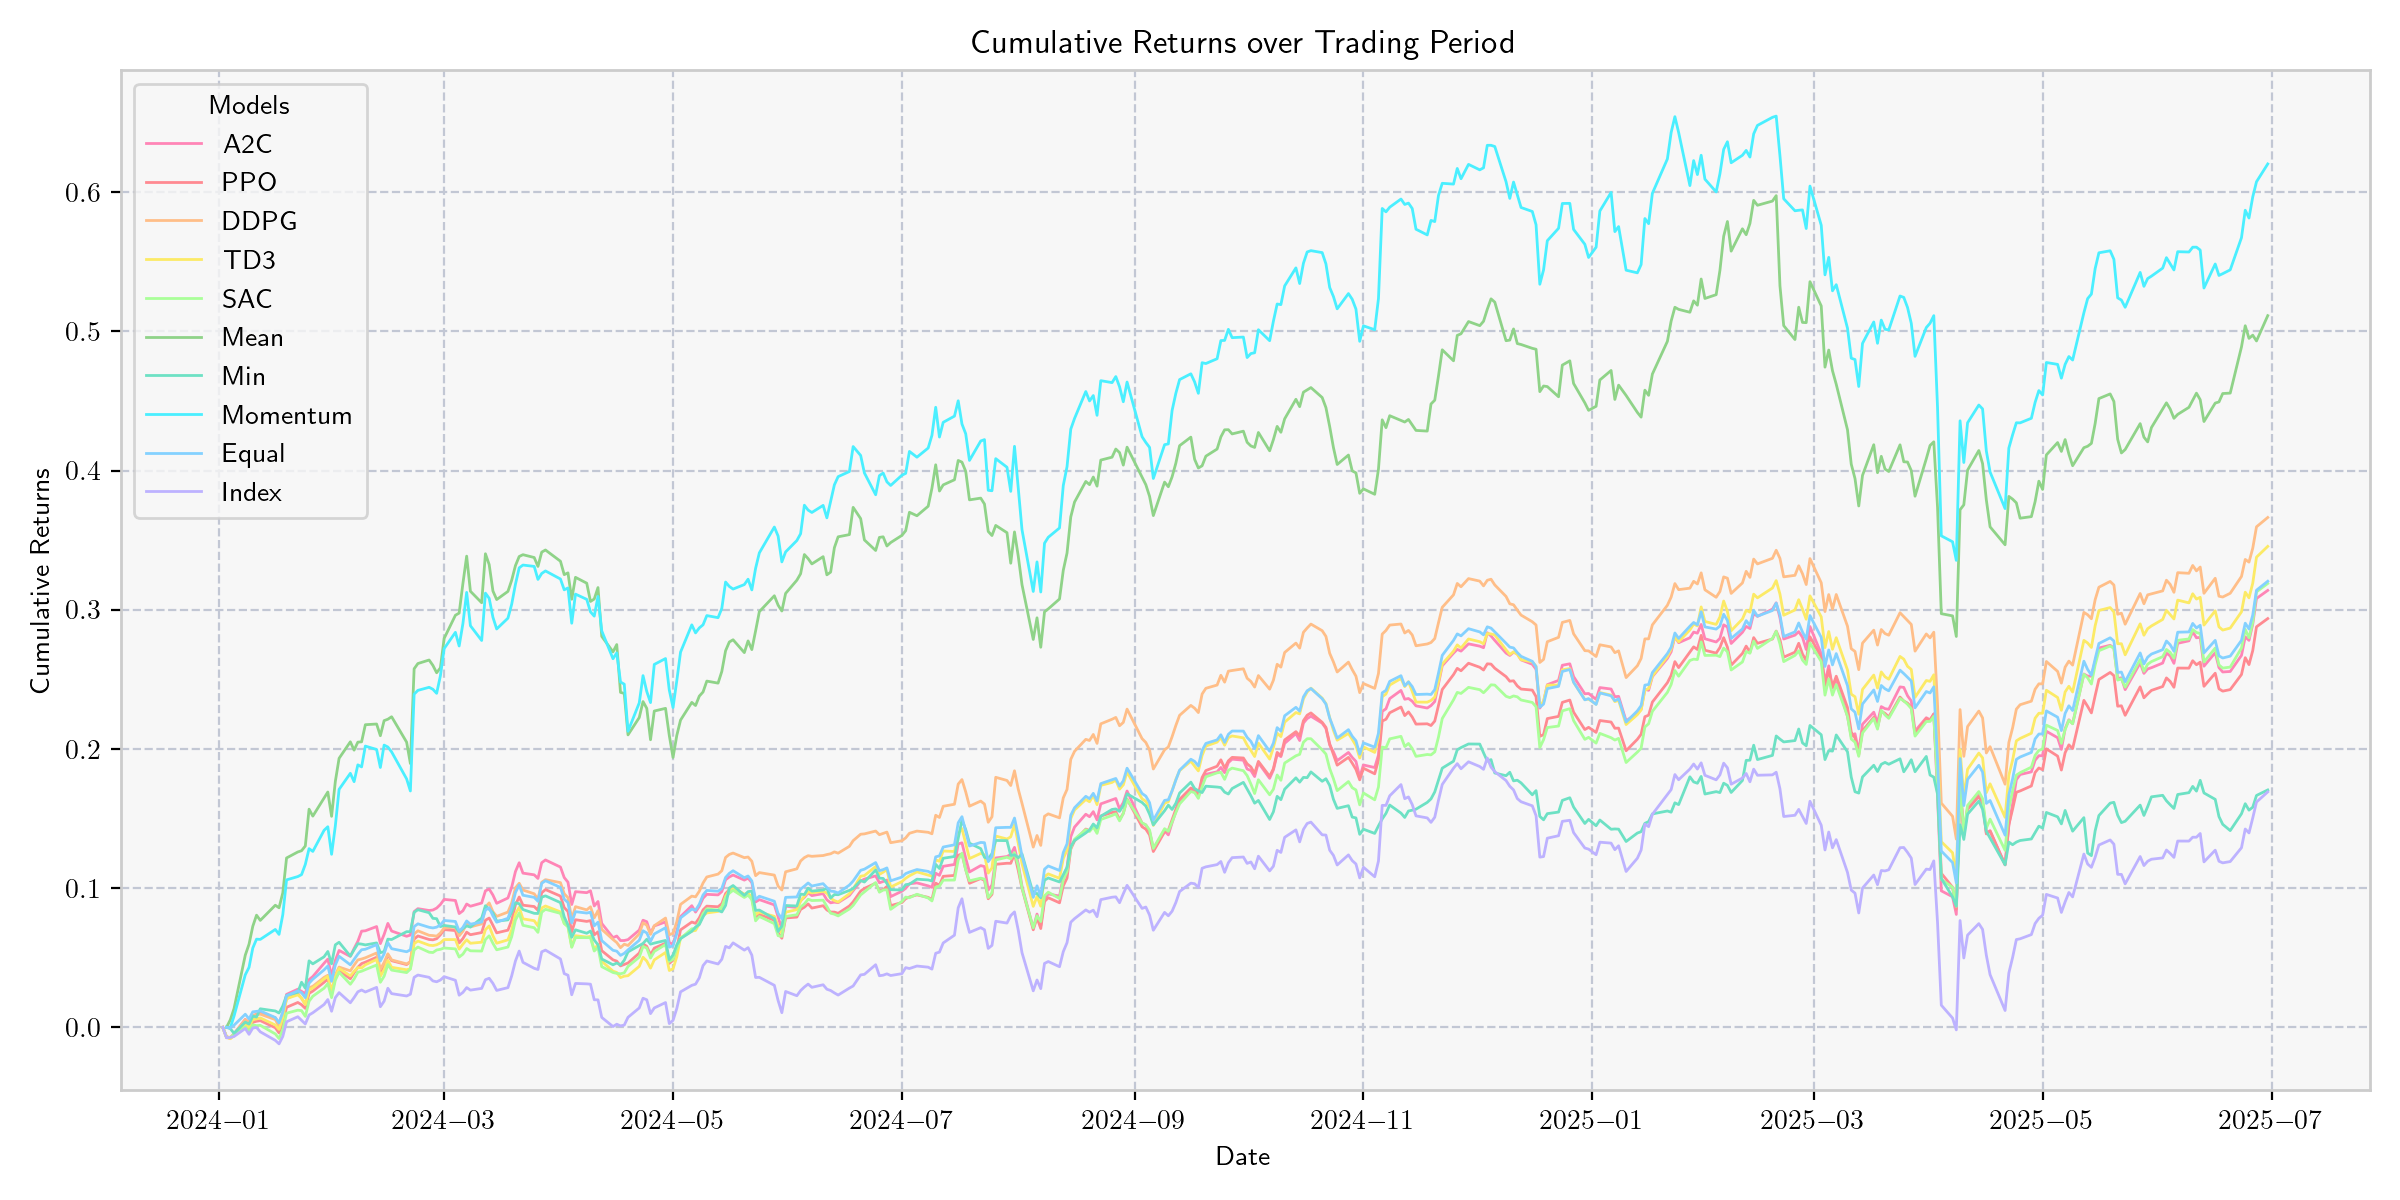
\includegraphics[width=\textwidth]{figures/dowjones30_indicators_cumulative_returns.png}
    \caption{Evolution of the Cumulative Returns for the DowJones30 dataset with the \acrshort{ohlcv} prices and indicators environment representation.}
    \label{fig:dowjones30_indicators_cumulative_returns}
\end{figure}

\begin{longtable}{|p{2cm}|p{2.1cm}|p{2.1cm}|p{2.1cm}|p{1.5cm}|p{2cm}|}
    \caption{Algorithm comparison results for the DowJones30 dataset. The colours correspond to the best performing configurations, with blue for the best performing \acrshort{drl} algorithm and green for the best benchmark.}
    \label{tab:experiment_algorithms_dow30} 
    \\ 
    \hline
    \textbf{Algorithm / Benchmark} & \textbf{Cumulative return} & \textbf{Annualised return} & \textbf{Annualised volatility} & \textbf{Sharpe ratio} & \textbf{Max drawdown}  \\ \midrule
    \endfirsthead

    \hline
    \textbf{Algorithm / Benchmark} & \textbf{Cumulative return} & \textbf{Annualised return} & \textbf{Annualised volatility} & \textbf{Sharpe ratio} & \textbf{Max drawdown}  \\ \midrule
    \endhead

    \endfoot
    \hline

    \textbf{A2C} & 0.2020 & 0.3139 & 0.1559 & 1.2575 & -0.1716 \\ \hline
    \textbf{PPO} & 0.1895 & 0.2937 & 0.1487 & 1.2407 & -0.1556 \\ \hline
    \textbf{DDPG} & \textcolor{blue}{0.2341} & 0.3663 & 0.1486 & \textcolor{blue}{1.4896} & -0.1546 \\ \hline
    \textbf{TD3} & 0.2214 & 0.3456 & 0.1517 & 1.3938 & -0.1609 \\ \hline
    \textbf{SAC} & 0.2050 & 0.3189 & 0.1480 & 1.3340 & -0.1538 \\ \midrule
    \textbf{Mean} & 0.3218 & 0.5114 & 0.1839 & 1.6096 & -0.1983 \\ \hline
    \textbf{Min} & 0.1123 & 0.1705 & 0.1157 & 0.9777 & -0.1066 \\ \hline
    \textbf{Momentum} & \textcolor{green}{0.3855} & 0.6204 & 0.1990 & \textcolor{green}{1.7388} & -0.1929 \\ \hline
    \textbf{Equal} & 0.2066 & 0.3205 & 0.1476 & 1.3461 & -0.1541 \\ \hline
    \textbf{Index} & 0.1110 & 0.1692 & 0.1532 & 0.7635 & -0.1637 \\ \hline
\end{longtable}

The results show that all the algorithms outperform the performance of the index for all the considered metrics, as well as the min-variance portfolio. Out of all the \acrshort{drl} algorithms, \acrshort{ddpg} achieves the highest cumulative return of 23.41\% and a Sharpe ratio of 1.49, followed by \acrshort{td3} with a cumulative return of 22.14\% and a Sharpe ratio of 1.39, while \acrshort{ppo} has the worst performance of the five with a cumulative return of 18.95\% and a Sharpe ratio of 1.24. However, none of these outperform the mean-variance and momentum benchmark strategies, with the latter achieving a Sharpe ratio of 1.74 and a cumulative return of 38.55\%, which is significantly higher than the performance of the \acrshort{drl} algorithms.

\section{Experiment: Environment Representation} \label{sec:environment-representation}

Another source of variability in the performance of the algorithms is the environment representation. In this section, the results of comparing the \acrshort{drl} algorithms on different environment representations are presented. For the experiment to be meaningful, it has been performed on the DowJones30 dataset, the currencies and the commodities datasets. This choice provides the ability to compare the performance of the algorithms across different asset classes, while also allowing for a more manageable computational cost. The table \ref{tab:experiment_environment_sharpe} compares the performance according to the Sharpe ratio and, in Appendix \ref{app:experiment_environment_representation}, according to the cumulative return.

\begin{longtable}{|p{2cm}|p{2.2cm}|p{2cm}|p{2cm}|p{2.2cm}|p{2cm}|}
    \hline
    \textbf{Algorithm} & \textbf{Dataset} & \textbf{Simple} & \textbf{Indicators} & \textbf{Covariance} & \textbf{Complete} \\ \midrule
    \endfirsthead

    \hline
    \textbf{Algorithm} & \textbf{Dataset} & \textbf{Simple} & \textbf{Indicators} & \textbf{Covariance} & \textbf{Complete}  \\ \midrule
    \endhead

    \caption{Environment representation experiment comparison according to the Sharpe ratio.}
    \label{tab:experiment_environment_sharpe}

    \endfoot

    \hline  
    \multirow{3}{*}{\textbf{A2C}}
    & DowJones30 & 1.3203 & 1.2575 & 1.3615 & \textcolor{blue}{1.3929} \\ \cline{2-6}
    & Commodities & 1.1373 & \textcolor{green}{1.2881} & 1.0273 & 1.2079 \\ \cline{2-6}
    & Currencies & -0.0018 & -0.0571 & -0.0674 & -0.0053 \\ \midrule

    \multirow{3}{*}{\textbf{PPO}}
    & DowJones30 & 1.3410 & 1.2407 & \textcolor{blue}{1.3524} & 1.1890 \\ \cline{2-6}
    & Commodities & \textcolor{green}{1.2600} & 1.1256 & 1.1559 & 1.2015 \\ \cline{2-6}
    & Currencies & 0.0014 & 0.0699 & 0.0652 & 0.1399 \\ \midrule

    \multirow{3}{*}{\textbf{DDPG}}
    & DowJones30 & 1.3826 & \textcolor{blue}{1.4896} & 1.3562 & 1.3261 \\ \cline{2-6}
    & Commodities & \textcolor{green}{1.1745} & 0.9871 & 1.0731 & 1.1612 \\ \cline{2-6}
    & Currencies & 0.0528 & 0.0689 & 0.0200 & 0.0115 \\ \midrule

    \multirow{3}{*}{\textbf{TD3}}
    & DowJones30 & \textcolor{blue}{1.4911} & 1.3938 & 1.1792 & 1.2084 \\ \cline{2-6}
    & Commodities & \textcolor{green}{1.4537} & 0.9776 & 1.0462 & 1.2388 \\ \cline{2-6}
    & Currencies & 0.0807 & -0.0088 & -0.0086 & -0.0436 \\ \midrule
    \pagebreak

    \multirow{3}{*}{\textbf{SAC}}
    & DowJones30 & 0.9769 & 1.3340 & \textcolor{blue}{1.4670} & 1.3017 \\ \cline{2-6}
    & Commodities & \textcolor{green}{1.3727} & 1.1973 & 1.1773 & 1.0500 \\ \cline{2-6}
    & Currencies & 0.0806 & 0.1771 & -0.1441 & 0.2550 \\ \midrule

\end{longtable}

The results show that the performance of the algorithms varies significantly across different environment representations. For the DowJones30 dataset, the \acrshort{ohlcv} prices representation achieves the highest Sharpe ratio of 1.49 for \acrshort{td3}, closely followed by the \acrshort{ohlcv} prices with indicators. The \acrshort{ohlcv} prices with covariance representation achieves 1.47 for \acrshort{sac}. For the complete feature set, only the \acrshort{a2c} algorithm achieves a higher Sharpe ratio of 1.39 than the other algorithms.

For the commodities dataset, the results are completely different to those of the DowJones30. The only coincidence is that \acrshort{td3} achieves the highest Sharpe ratio and highest cumulative return in the simple feature set. Moreover, when looking at this dataset, explicitly adding the covariance to the environment representation does not lead to better performance in terms of Sharpe ratio and there is only one instance where the cumulative returns are highest, which would be for the \acrshort{ddpg} algorithm with the complete feature set.

Finally, for the currencies dataset, the performance of the algorithms is significantly lower, going negative in some cases. A possible reason is the particular set of hyper-parameters used. In this experiment, algorithm configuration was not altered or tuned for each specific feature set.

\section{Experiment: Hyper-parameter Tuning} \label{sec:hyper-parameter-tuning}

As has been mentioned in the above experiments, the performance of the algorithms is substantially influenced by the choice of hyper-parameters. Ideally, a systematic approach should be employed to find the optimal hyper-parameters for each algorithm, dataset and environment representation combination. However, due to the computational cost of hyper-parameter tuning, it was only performed for the DowJones30 dataset with the \acrshort{ohlcv} and indicators environment representations over five trials. The results for each of the algorithms with the default hyper-parameters versus the tuned hyper-parameters are compared in Table \ref{tab:experiment_hyperparameters_simple} and Table \ref{tab:experiment_hyperparameters_indicators} for the two features sets: simple and with indicators, respectively.

\begin{longtable}{|l|l|l|l|}
    \caption{Hyper-parameter tuning experiment results for the DowJones30 dataset with simple feature set.}
    \label{tab:experiment_hyperparameters_simple}
    \\ 
    \hline
    \textbf{Algorithm} & \textbf{Metric} & \textbf{Default parameters} & \textbf{Tuned parameters} \\ \midrule
    \endfirsthead

    \hline
    \textbf{Algorithm} & \textbf{Metric} & \textbf{Default parameters} & \textbf{Tuned parameters} \\ \midrule
    \endhead

    \endfoot

    \multirow{2}{*}{\textbf{A2C}}
    & Cumulative Return & 0.3387 & 0.3491 \\ \cline{2-4}
    & Sharpe ratio & 1.3203 & \textcolor{blue}{1.4307} \\ \midrule

    \multirow{2}{*}{\textbf{PPO}}
    & Cumulative Return & 0.3174 & 0.2844 \\ \cline{2-4}
    & Sharpe ratio & \textcolor{blue}{1.3410} & 1.1939 \\ \midrule

    \multirow{2}{*}{\textbf{DDPG}}
    & Cumulative Return & 0.3454 & 0.27404 \\ \cline{2-4}
    & Sharpe ratio & \textcolor{blue}{1.3826} & 1.2088 \\ \midrule

    \multirow{2}{*}{\textbf{TD3}}
    & Cumulative Return & 0.3902 & 0.2974 \\ \cline{2-4}
    & Sharpe ratio & \textcolor{blue}{1.4911} & 1.2354 \\ \midrule

    \multirow{2}{*}{\textbf{SAC}}
    & Cumulative Return & 0.2243 & 0.3703 \\ \cline{2-4}
    & Sharpe ratio & 0.9769 & \textcolor{blue}{1.4521} \\ \midrule
\end{longtable}
\begin{longtable}{|l|l|l|l|}
    \hline
    \textbf{Algorithm} & \textbf{Metric} & \textbf{Default parameters} & \textbf{Tuned parameters} \\ \midrule
    \endfirsthead

    \hline
    \textbf{Algorithm} & \textbf{Metric} & \textbf{Default parameters} & \textbf{Tuned parameters} \\ \midrule
    \endhead

    \caption{Hyper-parameter tuning experiment results for the DowJones30 dataset with indicators environment representation.}
    \label{tab:experiment_hyperparameters_indicators}

    \endfoot

    \hline  
    \multirow{2}{*}{\textbf{A2C}}
    & Cumulative Return & 0.3139 & 0 \\ \cline{2-4}
    & Sharpe ratio & 1.2575 & 0 \\ \hline

    \multirow{2}{*}{\textbf{PPO}}
    & Cumulative Return & 0.2937 & 0 \\ \cline{2-4}
    & Sharpe ratio & 1.2407 & 0 \\ \hline

    \multirow{2}{*}{\textbf{DDPG}}
    & Cumulative Return & 0.3663 & 0 \\ \cline{2-4}
    & Sharpe ratio & 1.4896 & 0 \\ \hline

    \multirow{2}{*}{\textbf{TD3}}
    & Cumulative Return & 0.3456 & 0 \\ \cline{2-4}
    & Sharpe ratio & 1.3938 & 0 \\ \hline

    \multirow{2}{*}{\textbf{SAC}}
    & Cumulative Return & 0.3189 & 0 \\ \cline{2-4}
    & Sharpe ratio & 1.3340 & 0 \\ \hline
\end{longtable}

By looking at the data presented in these tables, it is clear that finding the optimal configuration can have a significant impact on the performance of the algorithms. For instance, although the cumulative return for \acrshort{a2c} in the simple feature set only improves by 1\%, the Sharpe ratio increases from 1.32 to 1.43, meaning that the algorithm learns to better balance risk while maximising returns. Another example is the \acrshort{sac} algorithm, which achieves a better performance than that of the default configuration. However, for the \acrshort{ppo}, \acrshort{ddpg} and \acrshort{td3} algorithms, there are no improvements and the default hyper-parameters perform better. Similarly, when looking at the indicators feature set, not all the algorithms show sign of improvements. These means that, for that particular algorithm, dataset and environment representation combination, the optimal hyper-parameter configuration has not been found. Understandably, due to the limited computational resources, the hyper-parameter search was very limited to only five runs, which is not sufficient for a thorough search.
